% A4縦・1段組の学習用（教科書風）
\documentclass[paper=a4,fleqn]{jlreq}
\special{papersize=\the\paperwidth,\the\paperheight}

\usepackage[margin=20truemm]{geometry}
\usepackage[dvipdfmx]{graphicx}
\usepackage{amsmath,amssymb}
\usepackage{tikz}
\usepackage{pgfplots}
\usepackage{etoolbox}
\usepackage{needspace}
\usepackage{bm}
\pgfplotsset{compat=1.18}
\usetikzlibrary{arrows.meta,calc,angles,quotes}

\preto{\section}{\needspace{0.35\textheight}}
\preto{\subsection}{\needspace{0.25\textheight}}

\ModifyHeading{section}{
  lines=1,
  before_space=14pt,
  after_space=6pt
}

\ModifyHeading{subsection}{
  lines=1,
  before_space=10pt,
  after_space=4pt
}

\title{3次元ベクトル}
\author{}
\date{}

\makeatletter
\renewcommand{\maketitle}{%
  \begin{center}
    {\large\bfseries \@title\par}
  \end{center}
  \vspace{4pt}
}
\makeatother

\newcommand{\formula}[1]{%
  \vspace{4pt}%
  \begin{center}{\large\bfseries\boldmath\(\displaystyle #1\)}\end{center}%
  \vspace{4pt}%
}

\begin{document}
\maketitle

\section{3次元ベクトルとは何か}

\subsection{2次元との違い}

2次元は \((x,y)\) で足りるが、3次元では \((x,y,z)\) が必要になる。高さが増えるだけで、考え方は同じである。

\begin{center}
\begin{tikzpicture}[scale=1.0,>=Stealth]
  \draw[->,gray!60] (0,0) -- (5.8,0) node[right] {$x$};
  \draw[->,gray!60] (0,0) -- (0,4.7) node[above] {$y$};
  \draw[->,gray!60] (0,0) -- (-1.4,-1.2) node[below left] {$z$};
  \draw[very thick,blue,->] (0,0) -- (4.1,2.8);
  \node[blue] at (4.2,3.1) {$\vec{a}$};
  \node at (2.2,0.7) {3次元は「横・縦・高さ」};
\end{tikzpicture}
\end{center}

\subsection{ゲームでの意味}

3次元では、キャラやカメラ、弾丸、敵の位置を空間中の点として扱う。上や下が入るので、2次元より現実に近い。

\textbf{大事：} 3次元になると、見た目の理解が少し難しくなる。そのぶん図で考える習慣が役に立つ。

\subsection{確認問題}
\begin{enumerate}
  \item 3次元で必要になる成分を答えよ。
  \item 2次元との違いを1つ述べよ。
  \item ゲームで3次元を使う例を1つ挙げよ。
\end{enumerate}

\section{成分表示と大きさ}

\subsection{成分表示}

3次元のベクトルは、3つの成分で表す。

\formula{\vec{a}=\begin{pmatrix}a_x\\a_y\\a_z\end{pmatrix}}

\subsection{大きさ}

3方向に伸びているので、長さは3つの2乗の和の平方根である。

\formula{|\vec{a}|=\sqrt{a_x^2+a_y^2+a_z^2}}

\textbf{例：} \(\vec{a}=\begin{pmatrix}1\\2\\2\end{pmatrix}\) なら、\(|\vec{a}|=3\) である。

\begin{center}
\begin{tikzpicture}[scale=0.95,>=Stealth]
  \draw[->,gray!60] (0,0) -- (6.0,0) node[right] {$x$};
  \draw[->,gray!60] (0,0) -- (0,4.6) node[above] {$y$};
  \draw[->,gray!60] (0,0) -- (-1.2,-1.0) node[below left] {$z$};
  \draw[very thick,blue,->] (0,0) -- (4.2,2.8);
  \draw[dashed,gray!60] (4.2,2.8) -- (4.2,0);
  \draw[dashed,gray!60] (4.2,2.8) -- (0,2.8);
  \node at (4.55,3.1) {$\vec{a}$};
  \node at (2.0,1.0) {2次元の図を少し立体的に考える};
\end{tikzpicture}
\end{center}

\subsection{単位ベクトル}

向きだけを使いたいときは、長さを1にする。

\formula{\hat{a}=\frac{\vec{a}}{|\vec{a}|}}

\subsection{確認問題}
\begin{enumerate}
  \item \(\vec{a}=\begin{pmatrix}2\\2\\1\end{pmatrix}\) の大きさを求めよ。
  \item \(\vec{b}=\begin{pmatrix}-1\\0\\0\end{pmatrix}\) の長さは何か。
  \item 単位ベクトルは何のために使うか。
\end{enumerate}

\section{足し算・引き算・スカラー倍}

\subsection{基本の計算}

3次元でも、やることは2次元と同じである。成分ごとに計算するだけ。

\formula{\vec{a}+\vec{b}=\begin{pmatrix}a_x+b_x\\a_y+b_y\\a_z+b_z\end{pmatrix}}

\formula{\vec{a}-\vec{b}=\begin{pmatrix}a_x-b_x\\a_y-b_y\\a_z-b_z\end{pmatrix}}

\formula{k\vec{a}=\begin{pmatrix}ka_x\\ka_y\\ka_z\end{pmatrix}}

\begin{center}
\begin{tikzpicture}[scale=0.95,>=Stealth]
  \draw[->,gray!60] (-0.5,0) -- (6.0,0) node[right] {$x$};
  \draw[->,gray!60] (0,-0.5) -- (0,4.4) node[above] {$y$};
  \draw[->,gray!60] (0,0) -- (-1.2,-1.0) node[below left] {$z$};
  \draw[very thick,blue,->] (0,0) -- (2.2,1.0) node[midway,above left] {$\vec{a}$};
  \draw[very thick,red,->] (2.2,1.0) -- (4.4,2.9) node[midway,right] {$\vec{b}$};
  \draw[very thick,teal!70!black,->] (0,0) -- (4.4,2.9) node[midway,above] {$\vec{a}+\vec{b}$};
\end{tikzpicture}
\end{center}

\subsection{ゲームでの見方}

位置に速度を足す、速度に加速度を足す、力を重ねる。考え方は全部同じである。

\subsection{確認問題}
\begin{enumerate}
  \item \(\vec{a}=\begin{pmatrix}1\\2\\3\end{pmatrix}\)、\(\vec{b}=\begin{pmatrix}3\\-1\\0\end{pmatrix}\) の和を求めよ。
  \item 同じく差を求めよ。
  \item \(2\vec{a}\) の意味を言葉で説明せよ。
\end{enumerate}

\section{内積と直交}

\subsection{内積}

3次元でも内積の形は同じである。

\formula{\vec{a}\cdot\vec{b}=a_xb_x+a_yb_y+a_zb_z}

\subsection{角度との関係}

\formula{\vec{a}\cdot\vec{b}=|\vec{a}||\vec{b}|\cos\theta}

\formula{\cos\theta=\frac{\vec{a}\cdot\vec{b}}{|\vec{a}||\vec{b}|}}

\subsection{直交判定}

\textbf{内積が0なら垂直である。} これは2次元でも3次元でも同じである。

\formula{\vec{a}\cdot\vec{b}=0 \iff \vec{a}\perp\vec{b}}

\begin{center}
\begin{tikzpicture}[scale=0.95,>=Stealth]
  \draw[->,gray!60] (0,0) -- (5.8,0) node[right] {$x$};
  \draw[->,gray!60] (0,0) -- (0,4.4) node[above] {$y$};
  \draw[->,gray!60] (0,0) -- (-1.2,-1.0) node[below left] {$z$};
  \draw[very thick,blue,->] (0,0) -- (4.0,1.0) node[midway,below right] {$\vec{a}$};
  \draw[very thick,red,->] (0,0) -- (1.2,3.4) node[midway,above left] {$\vec{b}$};
  \draw (1.0,0) arc[start angle=0,end angle=34,radius=1.0];
  \node at (1.3,0.45) {$\theta$};
\end{tikzpicture}
\end{center}

\subsection{確認問題}
\begin{enumerate}
  \item \(\vec{a}=\begin{pmatrix}1\\2\\3\end{pmatrix}\)、\(\vec{b}=\begin{pmatrix}4\\0\\-1\end{pmatrix}\) の内積を求めよ。
  \item \(\vec{a}=\begin{pmatrix}2\\1\\0\end{pmatrix}\)、\(\vec{b}=\begin{pmatrix}-1\\2\\0\end{pmatrix}\) は垂直か。
  \item 内積が0のとき、角度は何度か。
\end{enumerate}

\section{外積の再定義}

\subsection{まず2次元の外積を思い出す}

2次元では、外積を\textbf{数}として使った。向きと面積を知るための道具である。

\formula{\begin{pmatrix}a_x\\a_y\end{pmatrix}\times\begin{pmatrix}b_x\\b_y\end{pmatrix}=a_xb_y-a_yb_x}

\textbf{正なら反時計回り、負なら時計回り}である。

\subsection{3次元ではベクトルになる}

3次元では、外積は2本のベクトルの両方に垂直なベクトルになる。

\formula{\vec{a}\times\vec{b}=\begin{pmatrix}
 a_yb_z-a_zb_y\\
 a_zb_x-a_xb_z\\
 a_xb_y-a_yb_x
\end{pmatrix}}

\textbf{意味：} 面に垂直な向きを作るので、法線ベクトルとして使える。

\begin{center}
\begin{tikzpicture}[scale=0.95,>=Stealth]
  \draw[->,gray!60] (0,0) -- (5.5,0) node[right] {$x$};
  \draw[->,gray!60] (0,0) -- (0,4.2) node[above] {$y$};
  \draw[->,gray!60] (0,0) -- (-1.1,-0.9) node[below left] {$z$};
  \draw[very thick,blue,->] (0,0) -- (3.8,1.0) node[midway,below right] {$\vec{a}$};
  \draw[very thick,red,->] (0,0) -- (1.2,3.1) node[midway,left] {$\vec{b}$};
  \draw[very thick,teal!70!black,->] (0,0) -- (1.0,1.3) node[midway,above right] {$\vec{a}\times\vec{b}$};
  \draw[gray!50,dashed] (3.8,1.0) -- (4.9,4.1) -- (1.2,3.1);
  \node at (3.6,3.0) {外積は面に垂直};
\end{tikzpicture}
\end{center}

\subsection{大きさ}

外積の大きさは、2つのベクトルが作る平行四辺形の面積である。

\formula{|\vec{a}\times\vec{b}|=|\vec{a}||\vec{b}|\sin\theta}

\subsection{確認問題}
\begin{enumerate}
  \item 2次元の外積は何を表すか。
  \item 3次元の外積は何に垂直か。
  \item 外積の大きさは何を表すか。
\end{enumerate}

\section{面と法線}

\subsection{平面の考え方}

3次元では、1本のベクトルだけでなく、2本の独立なベクトルで面を表せる。

\formula{\vec{p}=\vec{p}_0+s\vec{u}+t\vec{v}}

\subsection{法線ベクトル}

面に垂直なベクトルを\textbf{法線ベクトル}という。外積で作れる。

\formula{\vec{n}=\vec{u}\times\vec{v}}

\subsection{反射の考え方}

壁に当たったときの跳ね返りは、法線ベクトルと内積で考えやすい。

\formula{\vec{r}=\vec{v}-2(\vec{v}\cdot\hat{n})\hat{n}}

\subsection{確認問題}
\begin{enumerate}
  \item 平面を表すのに、なぜ2本のベクトルが必要か。
  \item 法線ベクトルは何で求めるか。
  \item 反射の式に内積が入る理由を考えよ。
\end{enumerate}

\section{ゲーム開発への応用}

\subsection{3次元の位置更新}

ゲームでは、位置・速度・加速度をベクトルで持つと分かりやすい。

\formula{\vec{p}(t)=\vec{p}_0+t\vec{v}}

\formula{\vec{p}(t)=\vec{p}_0+t\vec{v}_0+\frac12t^2\vec{a}}

\subsection{球の衝突判定}

3次元では円の代わりに球を使う。考え方は2次元と同じである。

\formula{d<r_a+r_b}

\formula{d^2<(r_a+r_b)^2}

\begin{center}
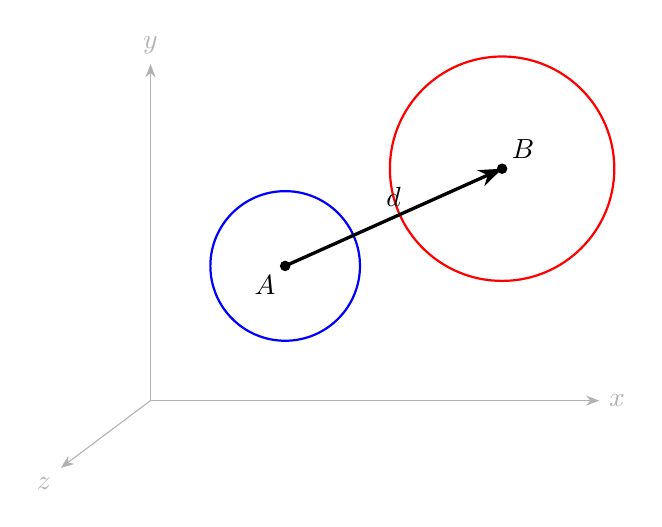
\begin{tikzpicture}[scale=0.95,>=Stealth]
  \draw[->,gray!60] (0,0) -- (6.0,0) node[right] {$x$};
  \draw[->,gray!60] (0,0) -- (0,4.5) node[above] {$y$};
  \draw[->,gray!60] (0,0) -- (-1.2,-0.9) node[below left] {$z$};
  \coordinate (A) at (1.8,1.8);
  \coordinate (B) at (4.7,3.1);
  \draw[thick,blue] (A) circle (1.0);
  \draw[thick,red] (B) circle (1.5);
  \fill (A) circle (2pt) node[below left] {$A$};
  \fill (B) circle (2pt) node[above right] {$B$};
  \draw[very thick,black,->] (A) -- (B) node[midway,above] {$d$};
\end{tikzpicture}
\end{center}

\subsection{ここで覚えること}

\begin{itemize}
  \item 2次元の考え方は、3次元でもほぼそのまま使える
  \item 3次元で新しく大事になるのは外積と法線である
  \item ゲームでは、当たり判定、面の向き、反射で役に立つ
\end{itemize}

\subsection{確認問題}
\begin{enumerate}
  \item 初期位置 \((0,0,0)\) 、速度 \((1,2,3)\) のとき、2秒後の位置を求めよ。
  \item 半径1と半径2の球の中心間距離が2.8なら、衝突しているか。
  \item 3次元で外積が重要になる理由を1つ挙げよ。
\end{enumerate}

\end{document}